\section{Tafeldetektion}

Das folgende Kapitel befasst sich mit dem ersten Schritt in der automatisierten Analyse der Grabungsfotos: der Erkennung der Schiefertafeln.\\
Zunächst werden die Tafeln vorgestellt und die Probleme bei der Detektion erörtert. Im Anschluss werden verschiedene Möglichkeiten der Erkennung präsentiert und diskutiert. Der Schwerpunkt liegt hier auf dem schlussendlich umgesetzten Verfahren.
Abschließend wird das mit der Tafeldetektion verbundene Ausschneiden der gefundenen Tafeln aus dem Gesamtbild vorgestellt.

\subsection{Einleitung: Die Tafeln}

Die Verwendung von Tafeln zur Dokumentation von Fund- und Grabungsarealen ist in allen, im weitesten Sinne grabenden, Wissenschaften weit verbreitet. So setzt auch die Archäologie diese Methode ein. Dabei werden neben den zu dokumentierenden Gebieten verschiedenste Formen von Tafeln oder Schildern platziert, auf denen Zeit und Ort der Aufnahme sowie weitere bild- und motivbezogene Informationen festgehalten werden können. Der Vielfalt von Form und Material der Tafeln ist dabei keine Grenze gesetzt.

\subsubsection{Die Tafeln als Ausgangsmaterial}

Bei den Tafeln, die Gegenstand dieses Projektes sind, handelt es sich um Schiefertafeln mit einem Holzrahmen, die mit Kreide beschriftet wurden (Vgl. Abb \ref{fig:einfachetafel}). Für die Detektion der Tafeln ergeben sich daraus folgende Faktoren:\\
\begin{enumerate}
\item Die Tafeln haben grundsätzlich eine rechteckige Form.
\item Durch die breite des Rahmens können bis zu zwei Rechtecke erkannt werden, ein Inneres und ein Äußeres.
\item Durch die große Differenz zwischen dem hellen Holzrahmen und der dunklen Schieferplatte sollte der innere Rand in der Regel gut detektierbar sein.
\end{enumerate}
\begin{figure}[!h]
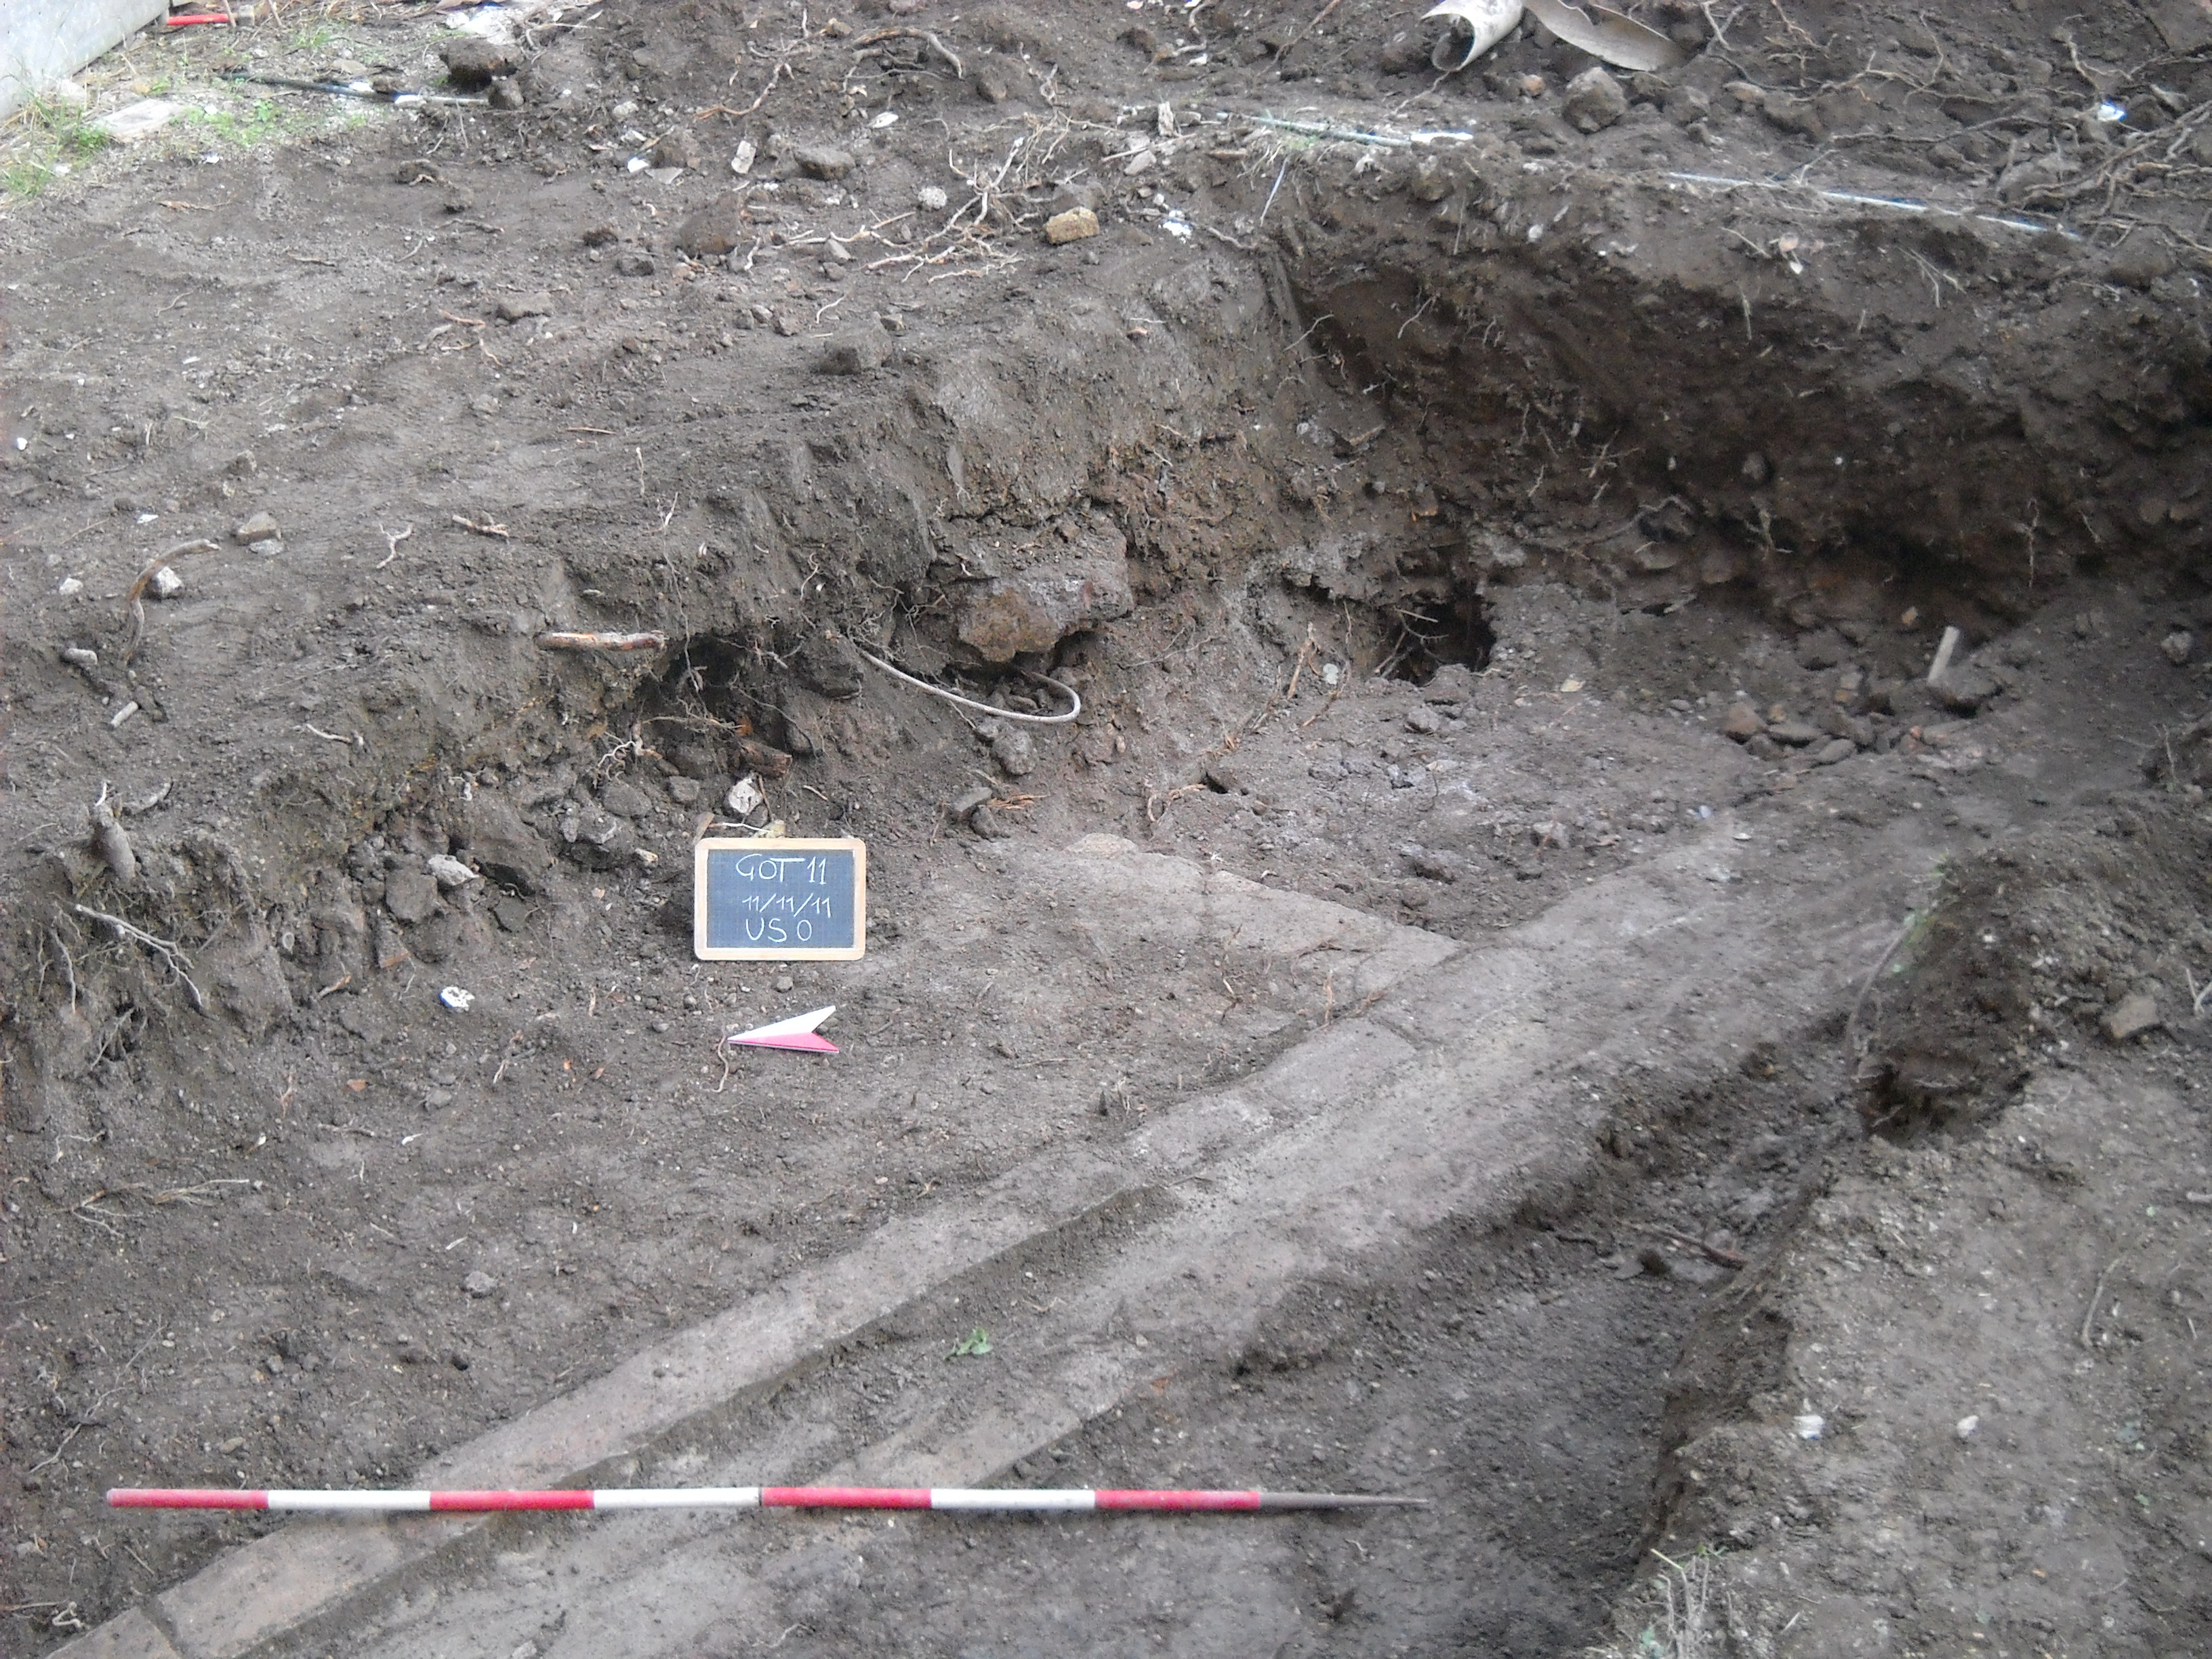
\includegraphics[width =0.5\textwidth]{catacom_1020.JPG}
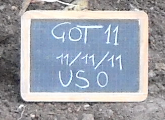
\includegraphics[width=0.5\textwidth]{catacom_1020_cutout.png}
\caption{Beispiel eines Fotos der verwendeten Tafel. GOT bezeichnet die Kampagne, darunter folgt das Datum. US ist die Abkürzung für \textit{unità stratigrafica}, die stratigrafische Einheit.}
\label{fig:einfachetafel}
\end{figure}
Die im Beispielbild gezeigte Tafel stellt  ein Idealbild dar: Die Tafel nimmt einen relativ großen Teil des Originalbildes ein. Sie ist frontal vor der Kamera positioniert. Die Beleuchtung ist gut und indirekt. Keines der weiteren Bildelemente verdeckt die Tafel.
Diese Beschreibung impliziert schon die Problemfelder, die bei der Detektion beachtet werden müssen:
\begin{enumerate}
\item Die Tafel ist unter Umständen stark rotiert (Vgl. Abb \ref{fig:schwierigetafel}).
\item Die Distanz der Tafel zur Kamera und damit ihre Größe im Bild kann stark variieren.
\item Der Rahmen der Tafel kann teilweise verdeckt oder anderweitig durch Gegenstände überlagert sein (Vgl. Abb \ref{fig:schwierigetafel}).
\item Die Farbe des Tafelrahmens kann dazu führen, dass sie sich nicht klar vom Hintergrund abhebt, was die Detektion des (äußeren) Randes erschweren kann.
\item Unregelmäßigkeiten im Rahmen, die auf grobe Verarbeitung oder Abnutzung zurückzuführen sind, können die Detektion erschweren.
\item Die Beleuchtung kann zu Problemen führen. Grundsätzlich sind alle Fotos hell und gut ausgeleuchtet, direktes Licht kann sich aber negativ auf die Kontraste auswirken.
\item Weitere Gegenstände, die den Spezifika der Tafeln entsprechen, können im Bild vorhanden sein.
\end{enumerate}
\begin{figure}[!h]
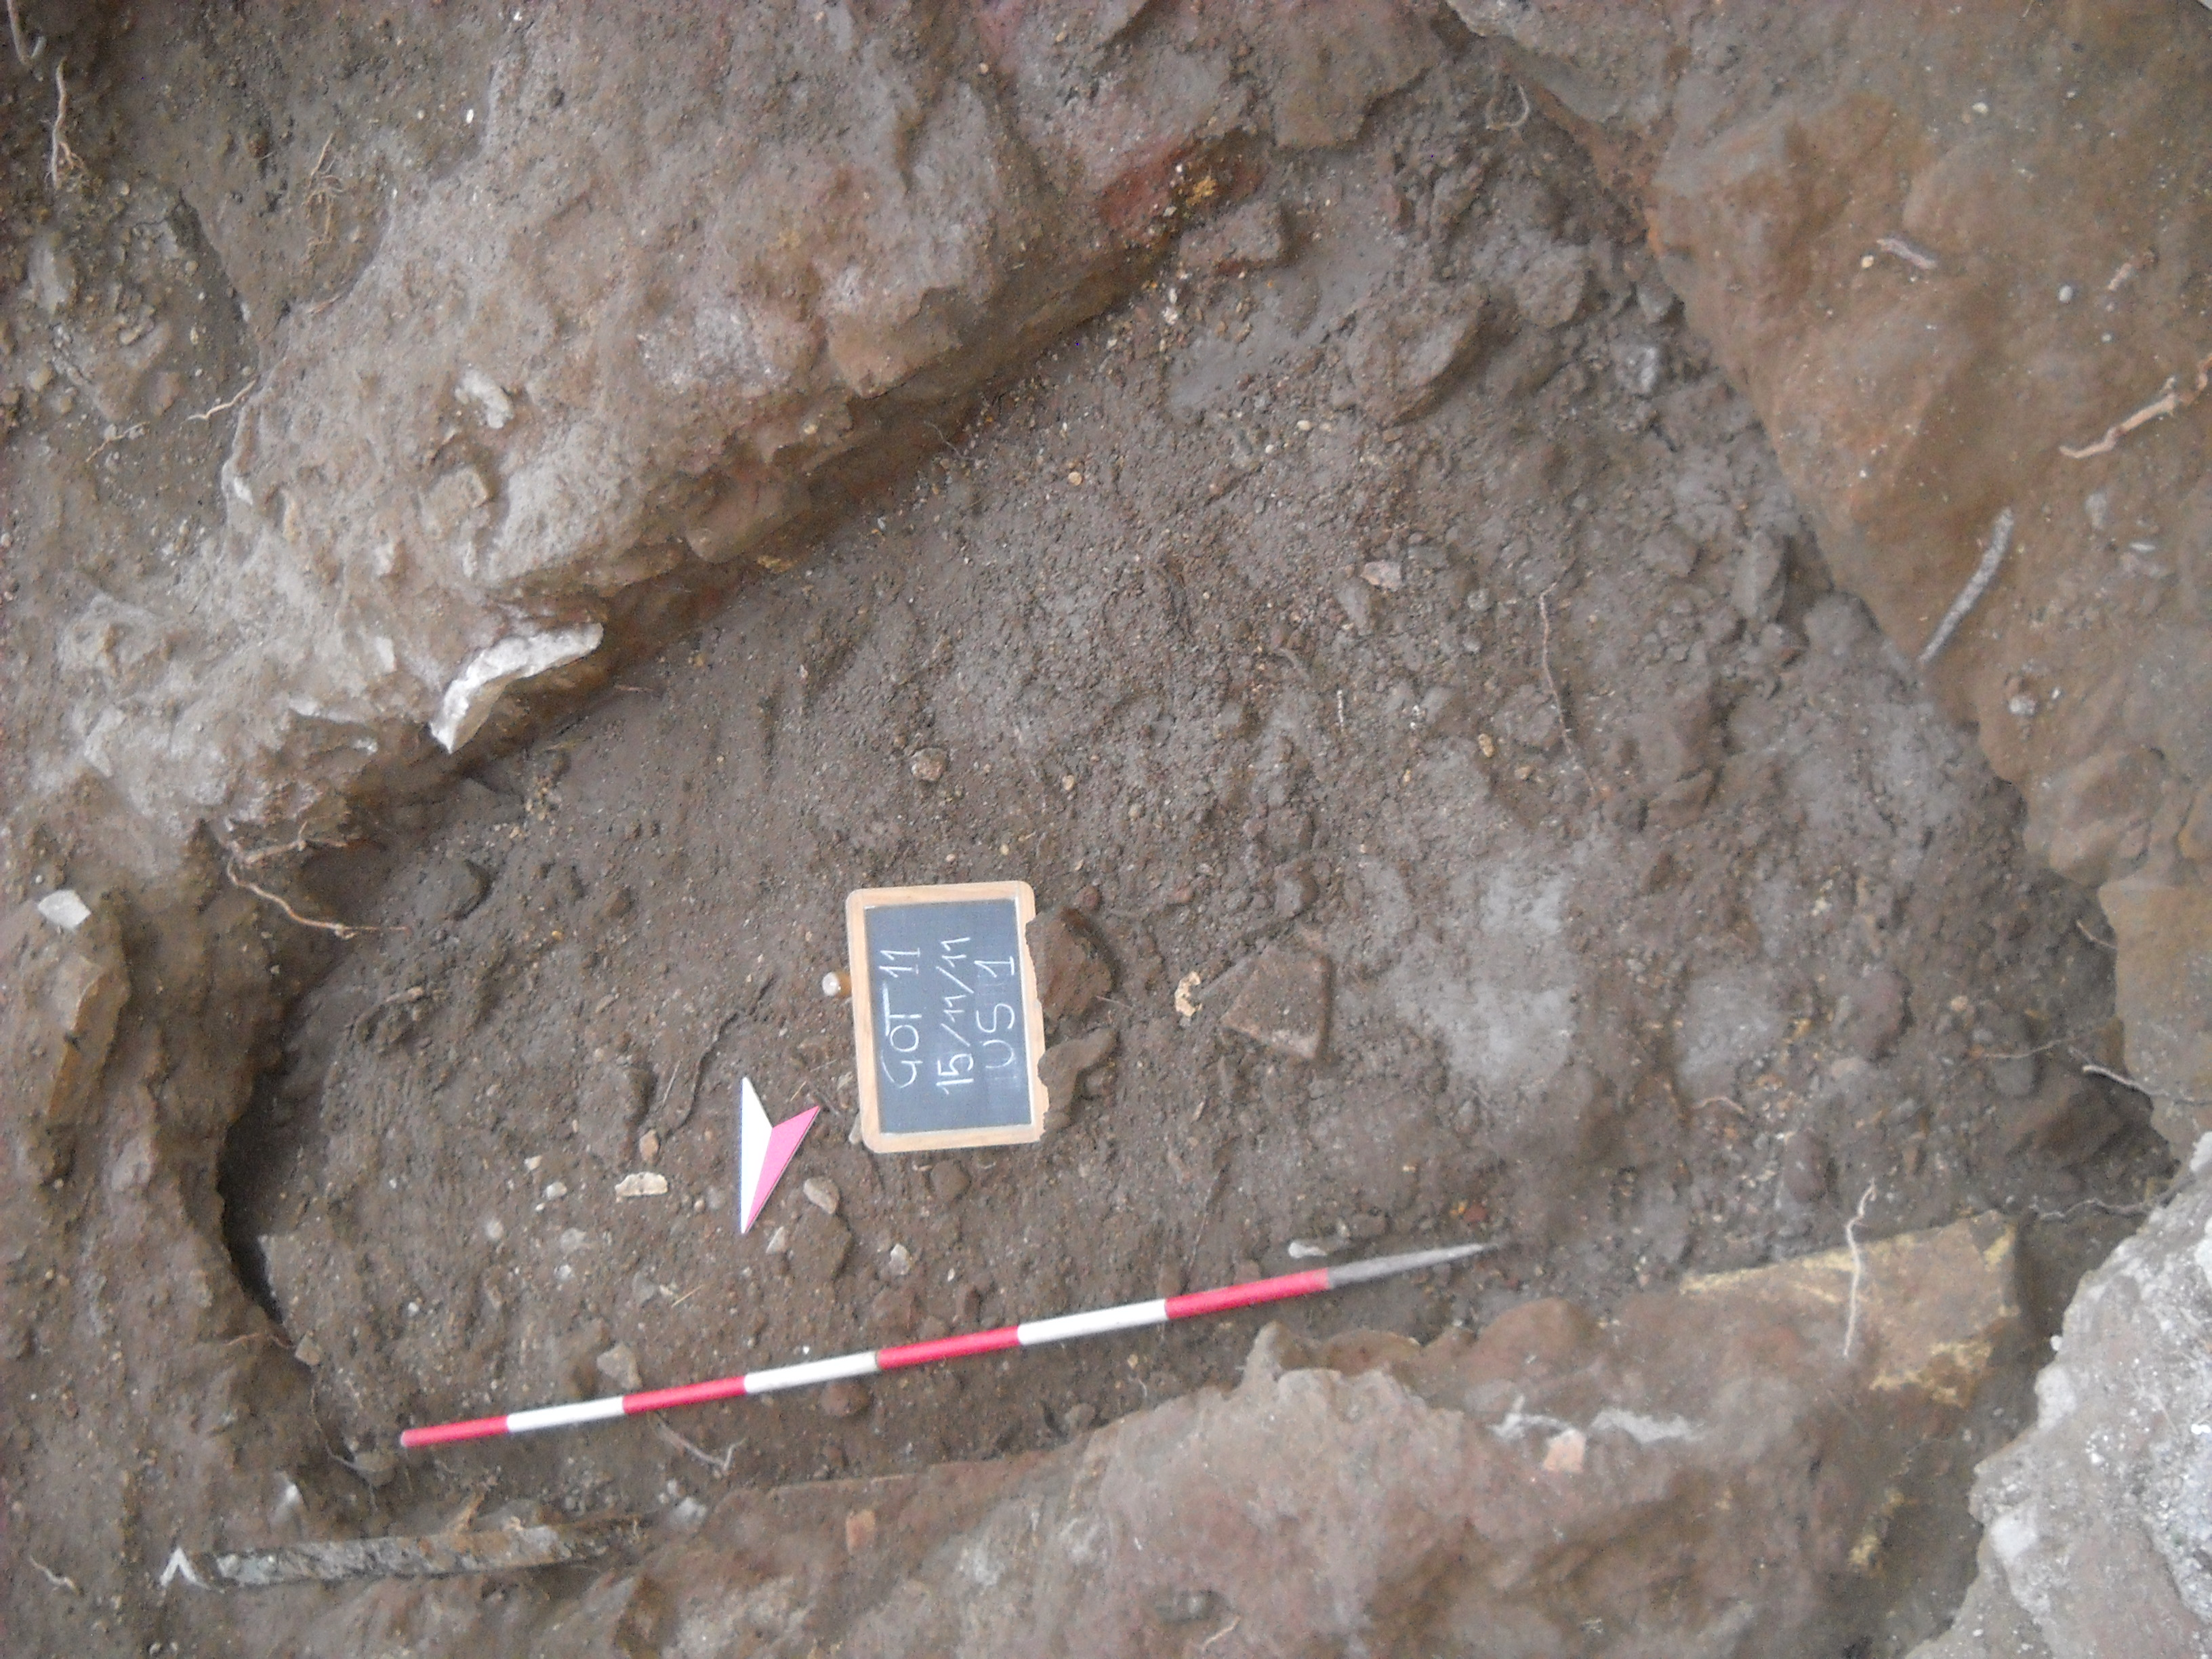
\includegraphics[width =0.5\textwidth]{catacom_1061_schwierige_tafel.JPG}
\caption{Schwierigere Detektion: Rotation und teilweise verdeckter Rahmen.}
\label{fig:schwierigetafel}
\end{figure}
Teilweise werden die hier genannten Probleme auch bei der Texterkennung wieder relevant. Auf diese und auf weitere wird an geeigneter Stelle zurückgegriffen.


\subsubsection{Tafelvergleiche}

Im Rahmen der Arbeit wurden weitere Tafeln exemplarisch dem Algorithmus unterzogen. Dabei handelte es sich um Aufnahmen der späteren Grabungen des Deutschen Archäologischen Institutes am Kapitol in Rom sowie um vergleichbare Fotos von Bodenuntersuchungen der Gruppe Terrestrische Ökohydrologie der Friedrich-Schiller-Universität Jena. Der ursprüngliche Gedanke dahinter war eine möglichst universale Detektion von Tafeln aller Art anzustreben. Die unterschiedlichen Daten konnten dabei vor allem Stärken und Schwächen der letztlich gewählten Technik aufzeigen.\\
Die Tafeln beider Projekte sollen im Folgenden kurz vorgestellt werden, um das Spektrum der Komplexität 
evtl. Vergleiche zu Tafeln aus späterer Grabung als Positivbeispiel:\\
besser gearbeitete Tafeln\\
besser lesbare Schrift\\
evtl. Vergleiche zu Tafeln der Bodenkunde als Negativbeispiel:\\
Tafel schwierig durch Form und Farbe\\
Klarsichthülle: Reflektion und Formveränderung\\
oft verdeckt\\
Bilder zur Veranschaulichung einfügen


\subsection{Detektionsverfahren}

Aus den oben genannten Punkten und den Anforderungen der Aufgabenstellung lässt sich als erster Arbeitsschritt die Detektion der Tafeln ableiten. Die wichtigste Prämisse ist dabei, dass Falsch-Negative, also nicht erkannte Tafeln, vermieden werden. Grund dafür ist, dass diese für die weitere Bearbeitung komplett verloren sind. Falsch-Positive sollten ebenfalls weitestgehend ausgeschlossen werden. Diese können jedoch in späteren Bearbeitungsschritten, bspw. der Texterkennung, erkannt und aussortiert werden. Daher ist dieses Kriterium von niedrigerer Priorität.
Dieses Kapitel wird sich daher verschiedenen Verfahren widmen, mit denen rechteckige, beschriftete Objekte erkannt werden können. Diese Verfahren werden kurz vorgestellt und ihre Ergebnisse in einer ersten, exploratorischen Umsetzung präsentiert. Anschließend wird begründet, warum diese Verfahren im Rahmen des Projektes nicht nicht zum Einsatz kamen. Final wird dann das Kontur-basierte Erkennungsverfahren erläutert, mit dem die besten Ergebnisse erzielt wurden.

%das Kapitel wird aus einer Kurzvorstellung der einzelnen Ansätze bestehen, die in Frage kamen und ausprobiert wurden
%In der Tiefe wird sich anschließend mit dem letztlich umgesetzten Verfahren, basierend auf \verb|cv2.contours|, auseinandergesetzt.

\subsubsection{Feature Detection}

was ist feature detection?
wie funktioniert sie?
was war die Idee hinter dem Ansatz?
Wie sehen die Ergebnisse aus?

\subsubsection{CNN}

hier werden CNNs vorgestellt
was sind CNNs?
Was können sie, wie funktionieren sie?
Warum habe ich sie ausprobiert, was war die Idee dahinter?
Warum habe ich nicht selbst trainiert?
Wie sehen die Ergebnisse aus?

\subsubsection{Contours}

was sind contours?
worin besteht die Grundidee?
wie wurde diese Idee umgesetzt? -> Flowchart
Zweispurigkeit der Ansätze: iterativ und adaptiv. Erklären warum.
\verb|rect_detect| als Finale, in dem die beiden Ansätze wieder zusammengeführt werden

\subsection{Cropverfahren}

Was ist die Aufgabe beim Crop?
Worin liegen hier die Schwierigkeiten?
Auch hier wieder Zweispurigkeit der Ansätze erklären

\subsubsection{simple crop}

Was ist die Idee?
Wie wurde sie umgesetzt?
Wo liegen die Probleme?

\subsubsection{Hough}

Was ist die Idee?
Wie wurde sie umgesetzt?
Wo liegen die Probleme?

\subsection{Zusammenfassung}
evtl zusammenfassen wie vorgegangen wurde, warum dieser Weg gut ist und was das Wichtigste Ergebnis ist